    \section{基态优势}
{\color{red}\begin{center}
    邱群、杨雅晴
    \end{center}}

    3.4.3节中的基态优势(Ground state dominance)近似是一种可以和平均场近似结合使用的非常有效的方法.
    当高分子聚合物限制在与$R_{g}$的尺度相比较小的区域上时,
    这种组合是比较合适的.
    我们通过回到现在所熟悉的正则系综中模型$A$的自由能问题泛函的推导来引入这个主题.
    \par
    正则模型$A$中的平均场公式(5.20)和(5.21)可以简便地重新表示成
    \label{subsec.equations}
    \begin{equation}
        \begin{aligned}
        \rho(r)=\hat{\rho}(\bm{r};[i\omega^{*}+J]),
            i\omega^{*}(\bm{r})=u_{0}\rho(\bm{r}). 
                   \end{aligned}
        \label{eq5.51}
    \end{equation}
    公式(3.167)和(4.75)可以进一步和基态优势近似结合将会得到
    \label{subsec.equations}
    \begin{equation}
        \begin{aligned}
            \rho(\bm{r})=\hat{\rho}(\bm{r};[i\omega^{*}+J])=nN[\psi(\bm{r})]^{2}.
                   \end{aligned}
        \label{eq5.52}
    \end{equation}
    公式中的基态特征函数$\psi(\bm{r})$满足公式(3.160)且$\omega\longrightarrow
    i\omega^{*}+J$, 即
    \label{subsec.equations}
    \begin{equation}
        \begin{aligned}
            \frac{b^2}{6}\nabla^{2}\psi(\bm{r})=[i\omega^{*}(\bm{r})+J(\bm{r})-\Lambda]\psi(\bm{r}).
                   \end{aligned}
        \label{eq5.53}
    \end{equation}
其中$\Lambda$是基态特征函数. 由外场$J$可以表示成
    \label{subsec.equations}
    \begin{equation}
        \begin{aligned}
            J[\rho]=\frac{b^{2}}{6\psi(\bm{r})}\nabla^{2}\psi(\bm{r})-u_{0}\rho+\Lambda.
                   \end{aligned}
        \label{eq5.54}
    \end{equation}
将这个结果代入公式(4.206)和(5.25)得到下面的密度泛函:
    \label{subsec.equations}
    \begin{equation}
        \begin{aligned}
            F[\rho]=\int d\bm{r}\
            \left(-\frac{nNb^{2}}{6}\psi\nabla^{2}\psi+\frac{u_{0}}{2}\rho^{2}-\Lambda\rho
            \right).
                   \end{aligned}
        \label{eq5.55}
    \end{equation}
其中项$-n\ln\ Q[i\omega^{*}+J]$被忽略了, 因为它比所示项的$O(1/N)$还要小.
\par
接下来的任务就是将公式(\ref{eq5.55})中包含$\psi$的项重新表示成$\rho$的泛函.
(\ref{eq5.52})微分产生$|\nabla\psi|^{2}=|\nabla\rho|^{2}/(4nN\rho)$,
将其代入(\ref{eq5.55})并分部积分会推出自由能泛函
    \label{subsec.equations}
    \begin{equation}
        \begin{aligned}
            F[\rho]=\int d\bm{r}\
            \left(\frac{b^{2}}{24\rho}|\nabla\rho|^{2}+\frac{u_{0}}{2}\rho^{2}-\Lambda\rho
            \right).
                   \end{aligned}
        \label{eq5.56}
    \end{equation}
在最后的这个表达式中, 保留了与$\Lambda$成比例的项.
或者$\Lambda$也可以被吸收在拉格朗日乘子(化学势)$\mu$中,
其在(4.202)中可以用来构造巨势$\Omega[\rho]$和加强限制$\int d\bm{r}=nN$.
\par
(\ref{eq5.56})给出的基态自由能泛函比(3.169)给出的泛函$F_{2}[\rho]$惊人地小.
事实上, 在$F_{2}[\rho]$代入$\omega\longrightarrow
i\omega^{*}/2=u_{0}\rho/2$会马上推出(\ref{eq5.56}).
从公式我们可以看到非均匀聚合物溶液的自由能泛函在基态可以近似作为$Lipshitz$熵项和平均场段与段之间反应项的和.
$Lipshitz$熵反应了与非均匀密度分布$\rho(\bm{r})$相关的构象熵惩罚.
\par
公式(\ref{eq5.56})和由慢梯度推导的自由能泛函(5.49)在形式上很相似.
在基态表达式中平移熵项$(\rho/N)\ln\rho$消失了, 当$N\longrightarrow \infty$,
或者$\xi/R_{g}\longrightarrow 0$是合理的,
其中$\xi$是聚合物位置所在区域的宽度. 
另外$Lifshitz$熵项的平方梯度系数在公式(5.49)中是$1/36$,
在公式$(\ref{eq5.56})$中是$1/24$. 这种矛盾的起源可以追溯到这样一个事实,
在尺度$R_{g}$上, $1/36$适用于缓慢密度变化, 而$1/24$则适用于快速密度变化.
事实上, 我们可以看到对于小振幅密度不均匀性,
慢梯度展开(5.49)中的系数$1/36$和$RPA$近似(5.27)对于$kR_{g}\ll 1$是保持一致的.
在快速密度变化的相反的极限, 即$kR_{g}\gg 1$,
在公式(\ref{eq5.56})$RPA$展开产生系数$1/24$. 换言之,
$RPA$和基态优势近似在小振幅上和在$R_{g}$尺度变换上大时是保持一致的.
然而基态表达式(\ref{eq5.56})并不局限于弱非均匀性.
\par
基态优势近似的第二个应用, 我们将考虑最初由$Helfand$和$Tagami$($Helfand\ and\ Tagami, 1971$)解决的对称聚合物与聚合物界面的经典问题.
他们研究了一类不可压共聚物混合模型的解析解,
这种模型是具有等统计段长度和聚合度的模型$C$的一种特殊的情况,
即$b_{A}=b_{B}=b$且$N_{A}=N_{B}=N$. 这个解依赖于平均场和基态优势近似.
其满足如果$\chi_{AB}\ll 1$, $N\gg 1$, 则$\chi_{AB}N\gg 1$. 强分离极限是指:
体系由两个在聚合物$A$和$B$中几乎纯的共存相组成, 通过一个窄的界面分开,
其宽度$\xi$比旋转半径$R_{g}=b(N/6)^{1/2}$要小的多.
\par
$Helfand$和$Tagami$考虑的情况对应于一个平面界面, 位于$z=0$处,
将在$z\longrightarrow +\infty$的$A$共聚物的纯相和在$z\longrightarrow
-\infty$的$B$共聚物的纯相分开. 平均场方程对应于
\label{subsec.equations}
    \begin{equation}
        \begin{aligned}
            \frac{\delta H[\omega_{\pm}]}{\delta
            \omega_{+}(z)}|_{\omega_{\pm}=\omega^{*}_{\pm}}=i\rho_{0}[\phi_{A}(z;
            [\omega^{*}_{A}])+\phi_{A}(z;
            [\omega^{*}_{A}])-1]=0.
                   \end{aligned}
        \label{eq5.57}
    \end{equation}
\label{subsec.equations}
    \begin{equation}
        \begin{aligned}
            \frac{\delta H[\omega_{\pm}]}{\delta
            \omega_{-}(z)}|_{\omega_{\pm}=\omega^{*}_{\pm}}=\rho_{0}[(2/\chi_{AB})\omega^{*}_{-}(z)-\phi_{A}(z;
            [\omega^{*}_{A}])+\phi_{A}(z;
            [\omega^{*}_{A}])]=0.
                   \end{aligned}
        \label{eq5.58}
    \end{equation}
其中$\omega_{A}=i\omega_{+}-\omega_{-}$,
$\omega_{B}=i\omega_{+}+\omega_{-}$是$A,B$单体的共轭化学势,
且$\phi_{K}$是$K$类单体的局部体积分数($K=A$或$B$), 由
\label{subsec.equations}
    \begin{equation}
        \begin{aligned}
        \phi_{K}(\bm{r}; [\omega_{K}])\equiv \hat{\rho}_{K}(\bm{r};
            [\omega_{K}])\rho_{0}.
        \end{aligned}
        \label{eq5.59}
    \end{equation}
这第一个平均场方程(\ref{eq5.57})表示了不可压缩条件,
即两种物质在每个位置的的体积分数之和必须为1. 第二个鞍点方程(\ref{eq5.58})表示,
交换化学势场和$A$类的体积分数有关,
在自洽场近似中$\omega^{*}_{-}(z)=\chi_{AB}[\phi_{A}(z; [\omega^{*}_{A}]-1/2)]$.
\par
方程(\ref{eq5.57})和(\ref{eq5.58})是一个难以处理的方程,
因其在鞍点$\omega^{*}_{\pm}(z)$处依赖与体积分数$\phi_{K}(z; [\omega^{*}_{K}])$.
然而, 利用基态优势近似, 体积分数可以简化成.
\label{subsec.equations}
    \begin{equation}
        \begin{aligned}
            \phi_{K}(z; [\omega^{*}_{K}])\approx[\psi_{K}(z)]^2.
        \end{aligned}
        \label{eq5.60}
    \end{equation}
其中基态特征函数$\psi_{K}(z)$满足
\label{subsec.equations}
    \begin{equation}
        \begin{aligned}
        \frac{b^{2}}{6}\frac{d^{2}}{dz^{2}}\psi_{A}(z)=[i\omega^{*}_{+}(z)-\omega^{*}_{-}(z)-\Lambda_{A}]\psi_{A}(z).
        \end{aligned}
        \label{eq5.61}
    \end{equation}
\label{subsec.equations}
    \begin{equation}
        \begin{aligned}
        \frac{b^{2}}{6}\frac{d^{2}}{dz^{2}}\psi_{B}(z)=[i\omega^{*}_{+}(z)+\omega^{*}_{-}(z)-\Lambda_{B}]\psi_{B}(z).
        \end{aligned}
        \label{eq5.62}
    \end{equation}
在这些方程中出现的基态特征值$\Lambda_{K}$的选择如下所述.
我们采用了与公式(3.161)不同的标准特征函数; 即$\int\
d\bm{r}\psi^{2}_{K}=V\phi_{K_{0}}$,
其中$\phi_{K_{0}}$是包含在体系中$K$类聚合物段的平均体积分数.
\par
在适当的边界条件下, 在两个共聚相之间可以形成一个单平面界面. 特别地,
当共存相是纯的时候, 正如渐进情况$\chi_{AB}N\longrightarrow \infty$,
有$\psi_{A}(+\infty)=\psi_{B}(-\infty)=1$,
$\psi_{A}(-\infty)=\psi_{B}(+\infty)=0$. 下面的梯度条件也适用于$K=A, B$:
$\psi^{'}_{K}(\pm\infty)=\psi^{"}_{K}(\pm\infty)=0$.
因为方程(\ref{eq5.61})和(\ref{eq5.62})是和边界条件是保持一致的,
必须满足$\Lambda_{A}=\Lambda_{B}=\Lambda$,
$i\omega_{+}(\pm\infty)-\chi_{AB}/2-\Lambda=0$.
可以选择一个简单的但任意的压力场$\omega_{+}(\pm\infty)=0$,
其暗示了$\lambda=-\chi_{AB}/2$. 因此方程(\ref{eq5.61})和(\ref{eq5.62})简化成
\label{subsec.equations}
    \begin{equation}
        \begin{aligned}
            \frac{b^{2}}{6}\frac{d^{2}}{dz^{2}}\psi_{A}(z)=[i\omega^{*}_{+}(z)+\chi_{AB}\phi_{B}(z)]\psi_{A}(z).
        \end{aligned}
        \label{eq5.63}
    \end{equation}
\label{subsec.equations}
    \begin{equation}
        \begin{aligned}
            \frac{b^{2}}{6}\frac{d^{2}}{dz^{2}}\psi_{B}(z)=[i\omega^{*}_{+}(z)+\chi_{AB}\phi_{A}(z)]\psi_{B}(z).
        \end{aligned}
        \label{eq5.64}
    \end{equation}
因此$A$聚合物段受到的平均势场是压力项$i\omega^{*}_{+}(z)$和$B$段局部接触反应项$\chi_{AB}\phi_{B}(z)$之和.
同样地$B$聚合物也受到相同的压力场, 但是反应势$\chi_{AB}\phi_{A}(z)$与$A$段的局部体积分数成比例
\par
$Helfand$和$Tagami$证明了当$K=A, B$时, 由\ref{eq5.57}),
(\ref{eq5.60})组成的五个方程对上述平面边界条件具有解析解, 这个解对应于
\label{subsec.equations}
    \begin{equation}
        \begin{aligned}
            \phi_{A}(z)=1-\phi_{B}(z)=\frac{1}{1+\exp{-z\xi}}.
        \end{aligned}
        \label{eq5.65}
    \end{equation}
\label{subsec.equations}
    \begin{equation}
        \begin{aligned}
            \psi_{K}(z)=[\phi_{K}(z)]^{1/2}.
        \end{aligned}
        \label{eq5.66}
    \end{equation}
\label{subsec.equations}
    \begin{equation}
        \begin{aligned}
            i\omega^{*}_{+}(z)=-3\chi_{AB}\phi_{A}(z)\phi_{B}(z).
        \end{aligned}
        \label{eq5.67}
    \end{equation}
其中$\xi$是界面宽度大小, 定义为
\label{subsec.equations}
    \begin{equation}
        \begin{aligned}
            \xi=\frac{b}{2(6\chi_{AB})^{1/2}}.
        \end{aligned}
        \label{eq5.68}
    \end{equation}
%\subsection{图像}
\label{subsec.figure}
\begin{figure}[htbp]
    \centering
%    \begin{minipage}[t]{0.2\linewidth}
    \centerline{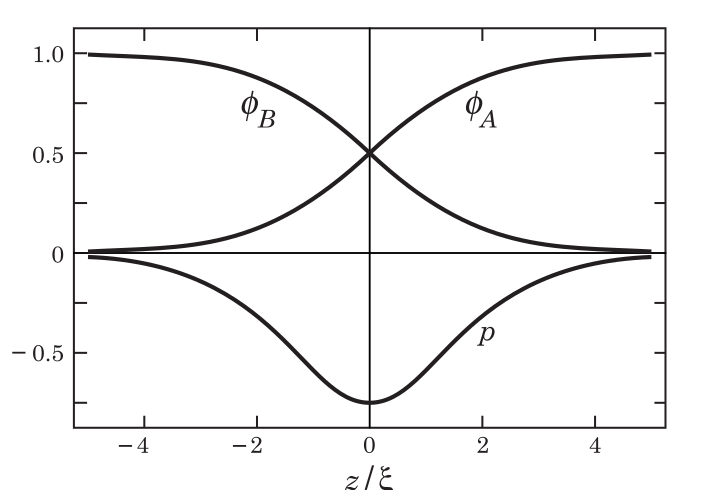
\includegraphics[scale=0.4]{./Contents/chapter5/figures/fig4.png}}
 %       \footnotesize{\centerline{(a)}}
 %   \end{minipage}
%    \hspace{0.2\linewidth}
%    \begin{minipage}[t]{0.2\linewidth}
%%        \centerline{\includegraphics[scale=0.4]{figure/figure2.png}}
%        \footnotesize{\centerline{(b)}}
%    \end{minipage}
    \caption{(书中的图5.4)\
    对称聚合物-聚合物界面的界面曲线的$Helfand-Tagami$解. $A,
    B$聚合物段的体积分数分别标记了$\phi_{A}$和$\phi_{B}$.
    整段的体积分数是单位1. $p$曲线表示压力场$p(z)\equiv
    i\omega^{*}_{+}(z)/\chi_{AB}$.}
	\label{fig.1}
\end{figure}




\par
与$Helfand-Tagami$解有关的平衡体积分数曲线$\phi_{A}(z)$和$\phi_{B}(z)$如图()所示.
界面宽度$\xi$与$A, B$所在区域宽度有关.
混合是与由$\chi_{AB}$参数化的$A-B$接触能相反的, 与扩散界面提供的构象熵成正比的.
压力场$i\omega^{*}_{+}(z)$是负的且位于界面区域. 场的作用将聚合物吸引到界面上,
从而在所有位置看来都是均匀的段密度.
\par
在章节$3.4.3$基态优势近似的有效性依赖于局部化学势域, 其远远小于$R_{g}$,
在本例中局部势就是压力场$i\omega^{*}_{+}(z)$,
不是约束整条链而是形成界面链段的环. 压力场的范围和界面宽度$\xi$是同阶的,
这个范围满足规则$\xi/R_{g}=1/[2(\chi_{AB}N)^{1/2}]\ll 1$, $\chi_{AB}N\gg 1$.
同样地, 平均场近似的有效性要求$C\gg 1$, 其中$C$是公式(5.5)定义的配位数.
因为在熔融状态下$C\sim \rho_{0}b^{3}N^{1/2}$, 只要$A$和$B$都是高分子量的,
这个条件就满足了, 即$N\gg 1$. 最后, 为使$Helfand-Tagami$解是有效的,
界面宽度$\xi$必须不能低于介观尺度. 换言之, 必须有$\xi\gg
b$,或等价地$\chi_{AB}\ll 1$. 只要满足条件$\chi_{AB}\ll 1$和$\chi_{AB}N\gg
1$,我们就认为$Helfand-Tagami$解是准确的. 
\par
非常重要的是我们要注意到公式(\ref{eq5.68})描述的的是固有的界面宽度,
在流体-流体界面实验中测量了界面宽度, 它包含了界面的长波长表面波动张力,
因此超出了固有界面宽度(Weeks,\ 1977;\ Huse\ et\ al.,\ 1985;\ Binder\ et\ al.,\
2001). 这样的表面波动张力可以被看作是一种特殊的场波动, 尤其是对与层几何.
\par
对称聚合物-聚合物界面的表面张力可以由$Helfand-Tagami$解获得,
注意到张力是每单位表面面积多余的自由能(Chandler,\ 1987), 且在平均场近似中,
$A(n_{A},\ n_{B},\ V,\ T)\approx k_{B}T\ H[\omega^{*}_{+},\ \omega^{*}_{-}]$.
通过公式(4.98), 界面张力可以由

\label{subsec.equations}
    \begin{equation}
        \begin{aligned}
            \gamma&=k_{B}T\rho_{0}\int^{+\infty}_{-\infty}\ dz\left(
            \frac{1}{\chi_{AB}}[\omega^{*}_{-}(z)]^{2}-i\omega^{*}_{+}(z)-\frac{1}{4}\chi_{AB}\right),
            \\
            &=-k_{B}T\rho_{0}\int^{+\infty}_{-\infty}\ dz\ (
            \chi_{AB}\phi_{A}(z)\phi_{B}(z)+i\omega^{*}_{+}(z)),
            \\
            &=2k_{B}T\rho_{0}\chi_{AB}\int^{+\infty}_{-\infty}\ dz\
            \phi_{A}(z)\phi_{B}(z),
            \\
            &=k_{B}T\rho_{0}(\chi_{AB}/6)^{1/2}.
        \end{aligned}
        \label{eq5.69}
    \end{equation}
因此强分离聚合物-聚合物界面的表面张力是与聚合物分子量无关的,
它的尺度是$Flory$相互作用参数$\chi_{AB}$的平方根.
\par
一个简单的缩放参数可以用来更好的理解公式(\ref{eq5.68})和(\ref{eq5.69}).
正如图(5.5)所示, 界面区域可以看作是相互混合的环的区域的宽度.
界面宽度$\xi$可以表示环路相互混合的区域的宽度.
考虑一个典型的包含$g$统计段的环, $g$的值可以看作是均分估计, 即:
一个环表示一条链对不同聚合物相的相互渗透,
这种渗透只能在成本为$O(k_{B}T)$的情况下才能发生.
带有$g$个段的环的能量损耗是$\sim g\chi_{AB}k_{B}T$, 因此我们可以得出结论$g\sim
1/\chi_{AB}$. 当$\chi_{AB}\ll 1$时, 这是一个很大的数.
因为的每个环的强作用力只与热能尺度有关系,
界面宽度可以估计成一个未受干扰的$g$段聚合物的大小, 即: $\xi\sim bg^{1/2}\sim
b/\chi_{AB}^{1/2}$. 这个尺度很显然是与公式(\ref{eq5.68})是保持一致的. 最后,
界面张力可以估计成由$A-B$接触引起的界面多余自由能密度($\sim
k_{B}T\rho_{0}\chi_{AB}$)乘以区域宽度$\xi$,即得到公式$\gamma\sim
k_{B}T\rho_{0}b\chi_{AB}^{1/2}$.
这个结果很显然是与公式(\ref{eq5.69})是保持一致的.

\label{subsec.figure}
\begin{figure}[htbp]
    \centering
%    \begin{minipage}[t]{0.2\linewidth}
    \centerline{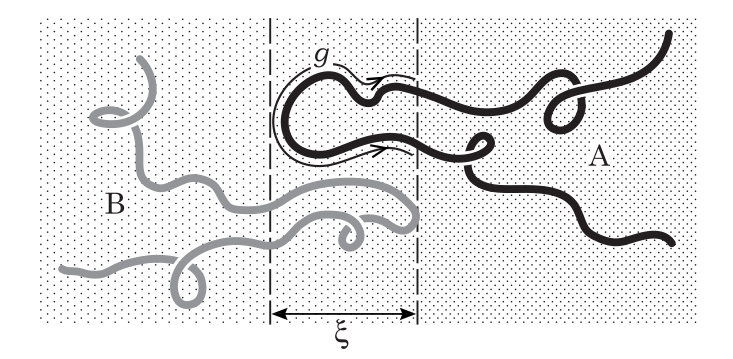
\includegraphics[scale=0.4]{./Contents/chapter5/figures/fig5.png}}
 %       \footnotesize{\centerline{(a)}}
 %   \end{minipage}
%    \hspace{0.2\linewidth}
%    \begin{minipage}[t]{0.2\linewidth}
%%        \centerline{\includegraphics[scale=0.4]{figure/figure2.png}}
%        \footnotesize{\centerline{(b)}}
%    \end{minipage}
    \caption{(书中的图5.5)\ 聚合物-聚合物界面的链构象示意图.
    一条穿过界面的聚合物链贡献了带有$g$段的环.
    且$A$环和$B$环混合穿过宽度为$\xi$的区域.}
	\label{fig.2}
\end{figure}



\subsubsection{强拉伸}
里另外一个有效的技术就是(3.4.4.2)节中描述的"强拉伸"近似与平均场近似的组合.阐释这种方法的一个有用的背景就是用模型$K$描述的溶液聚合物刷.
在足够高的密度系链下,刷中的聚合物被强烈拉伸, 可以采用这种经典的近似.
\par
在平均场近似中, (实数)势$\mu(z)\equiv
i\omega^{*}(z)$和平均段密度$\rho_{z}\equiv \hat{\rho}(z;
[i\omega^{*}])$在刷中每一个位置处成立关系
\label{subsec.equations}
    \begin{equation}
        \begin{aligned}
          \mu(z)=u_{0}\rho(z).
        \end{aligned}
        \label{eq5.70}
    \end{equation}
其中采用的是图(4.7)中的坐标体系. 经典的路径$z(s)$开始与嫁接面$z(0)=0$,
终止与$z(N)=z_{0}$, 满足公式(3.194), 即
\label{subsec.equations}
    \begin{equation}
        \begin{aligned}
            \frac{3}{b^{2}}\frac{d^{2}}{ds^{2}}z(s)=\frac{d\mu(z(s))}{dz(s)}.
        \end{aligned}
        \label{eq5.71}
    \end{equation}
其中尺寸单位已经恢复了. 因为不管末端位置是什么, 刷中所有的链都具有$N$个统计段,
"等时间限制"说明$\mu(z)$经典的近似必须是调和势, 即$\mu(z)=C_{1}-C_{2}z^{2}$.
带有这样的调和势, 并带有条件$z(0)=0$, $z(N)=z_{0}$,
且$[dz(s)/ds]_{s=N}=0$(在自由链端没有张力), 方程(\ref{eq5.71})可以求解出来.
经典路径
\label{subsec.equations}
    \begin{equation}
        \begin{aligned}
            z(s)=z_{0}\sin(\pi s/(2N)).
        \end{aligned}
        \label{eq5.72}
    \end{equation}
平方项系数
\label{subsec.equations}
    \begin{equation}
        \begin{aligned}
            C_{2}=\frac{3\pi^{2}}{8b^{2}N^{2}}.
        \end{aligned}
        \label{eq5.73}
    \end{equation}
第二个系数$C_{1}$可以通过保持分段关系
\label{subsec.equations}
    \begin{equation}
        \begin{aligned}
            \sigma N=\int^{h}_{0}dz\ \rho(z)=u_{0}^{-1}\int^{h}_{0}dz\
            (C_{1}-C_{2}z^{2}).
        \end{aligned}
        \label{eq5.74}
    \end{equation}
其中$h=(C_{1}/C_{2})^{1/2}$是聚合物刷厚度, 定义$\rho(h)=0$.
公式(\ref{eq5.74})的相当于是
\label{subsec.equations}
    \begin{equation}
        \begin{aligned}
            C_{1}=\frac{\sigma u_{0}N}{h}+\frac{C_{2}h^{2}}{3}.
        \end{aligned}
        \label{eq5.75}
    \end{equation}
通过组合这些结果, 我们得到了一个关于平衡刷厚度的重要公式(Milner\ et\ al., 1988)
\label{subsec.equations}
    \begin{equation}
        \begin{aligned}
            h=(\frac{4}{\pi^{2}})^{1/3}(\sigma u_{0})^{1/3}b^{2/3}N.
        \end{aligned}
        \label{eq5.76}
    \end{equation}
这公式有效的一个标准是聚合物被拉伸到一个高度,
其远远超过了它们未受干扰的尺度,$h/R_{g}\gg 1$. 相当于$(\sigma
u_{0}/b)^{1/3}N^{1/2}\gg 1$, 或者等价于$(\sigma R^{2}_{g})B\gg 1$,
其中$B$是由(5.28)定义的无量纲体积分数参数.
我们将可以看到参数$B$将在第六章中, 在聚合物溶液中评估排除体积效应的强度起到一个重要的作用. 
\par
在平均场密度近似和强拉伸近似的组合中,
平衡段密度曲线$(u_{0}/C_{1})\rho(z)=1-(z/h)^{2}$在图(5.6)中画出来了.
这个抛物曲线反应了在高嫁接密度时平均场段密度分布(Milner, 1990). 然而,
图中的虚线显示, 强拉伸近似对平均场曲线的近似并不是一致有效的,
在表面和刷的外边界周围都是由偏差的.
在$z=0$附近的耗长边界层已经在(4.9.4)讨论过了. 事实上,
带有适用于在$z=0$的传播子的$Dirichlet$条件的模型$K$的全平均场的解显示了一个尖锐层,
正如图(5.6)的虚线所示. 密度梯度随着嫁接的密度的增大而增大.
从图我们可与清晰地看到, 强拉伸近似只适用于边界层外, 其中$\mu(z)$缓慢变化,
且在$z=0$处符合黎曼边界条件. 同样地, 在刷的外边界,
平均场方程的近似解表现了密度曲线的缓慢变化(Milner, 1990),
与突然终止与$z=h$的抛物曲线相反. 外边界层是由于在刷子边缘的强烈拉伸引起的,
这个区域h中, 平均密度曲线是多个聚合物构象的结果.
$Matsen$最近对于"干聚合物刷"的强拉伸近似和平均场近似之间,
以及在干刷和化学性质相同的均聚物熔体之间的界面做了相似的比较(Matsen, 2004;
Matsen, 2005a).


\label{subsec.figure}
\begin{figure}[htbp]
    \centering
%    \begin{minipage}[t]{0.2\linewidth}
    \centerline{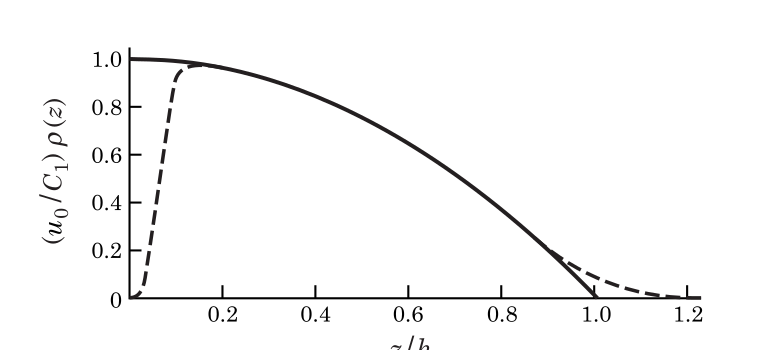
\includegraphics[scale=0.4]{./Contents/chapter5/figures/fig6.png}}
 %       \footnotesize{\centerline{(a)}}
 %   \end{minipage}
%    \hspace{0.2\linewidth}
%    \begin{minipage}[t]{0.2\linewidth}
%%        \centerline{\includegraphics[scale=0.4]{figure/figure2.png}}
%        \footnotesize{\centerline{(b)}}
%    \end{minipage}
    \caption{(书中的图5.6)\
    聚合物刷的模型$K$的平均场近似和强拉伸近似组合得到的段密度曲线$\rho(z)$的示意图.
    在高嫁接密度下, 实曲线表示全平均场密度分布, 边界层如虚线所示. 在表面附近,
    经典近似采用黎曼边界条件且忽略了狭窄的耗尽层. 在刷的外边界,
    强拉伸近似衰弱下来形成了一条光滑额曲线.}
	\label{fig.3}
\end{figure}



\par
模型$K$的强拉伸理论和全平均场解都忽略了场波动. 在嫁接点$\sim\sigma^{1/2}$, 当短波长低于平均间距的情况下,
场波动是最强烈的, 且引起了刷的不能在平均场近似中看到的一个局部的排除体积效应.
排除体积效应可以通过利用"斑点事件"近似地纳入平均场理论中(Milner\ et\ al, 1988;
Netz\ and\ Schick, 1988), 但是完全处理需要通道第六章中的数值方法. 和本节相关的,
我们将注意到经典近似中的已经被$Semenov$证明的一个有力的静电类比(Semenov,
1985). 这个类比已经被证实对非均匀聚合物的各种计算是非常有效的,
其中强链拉伸的假设是合理的(Semenov, 1985; Zhulina\ et\ al, 1992; Fredrickson\
et\ al., 1992).




%文章引用\,\cite{,}.
%\subsection{方程}
%\label{subsec.equations}
%\begin{itemize}
%	\item[$\bullet$] 示例 1
%	\begin{equation}
%		\begin{aligned}
%			a = b,
%			\\
%			b = c.
%		\end{aligned}
%		\label{eq.1}
%	\end{equation}
%	\item[$\bullet$] 示例 2
%	\begin{equation}
%		\left\{
%		\begin{aligned}
%			a = b,
%			\\
%			b = c.
%		\end{aligned}
%		\right.
%		\label{eq.2}
%	\end{equation}
%\end{itemize}
%
%
%\subsection{表格}
%\label{subsec.table}
%%% A, a, I, i, 1
%%% \Alph, \alph, \Roman, \roman, \arabic
%\begin{enumerate}[(I)]
%	\item 示例 1
%	\begin{table}[htbp]
%		\centering
%		\caption{表格示例}
%		\label{tab.1}
%		%% set the width of each column;
%		\begin{tabular}{p{3.5cm}|p{2cm}|p{5cm}<{\centering}}
%			\hline
%			a &b &c\\
%			\hline
%		\end{tabular}
%	\end{table}
%\end{enumerate}
%
%
%\subsection{图像}
%\label{subsec.figure}
%\begin{figure}[htbp]
%    \centering
%    \begin{minipage}[t]{0.2\linewidth}
%%        \centerline{\includegraphics[scale=0.4]{figure/figure1.png}}
%        \footnotesize{\centerline{(a)}}
%    \end{minipage}
%    \hspace{0.2\linewidth}
%    \begin{minipage}[t]{0.2\linewidth}
%%        \centerline{\includegraphics[scale=0.4]{figure/figure2.png}}
%        \footnotesize{\centerline{(b)}}
%    \end{minipage}
%    \caption{图像示例}
%	\label{fig.1}
%\end{figure}
%


%\section*{致谢} 

%%% 附录;
%    \newpage
%\begin{appendix}
%    \section{附录}
%    公式的推导.
%\end{appendix}


%\bibliography{ref}
%\bibliographystyle{unsrt}


